\section*{Lab activity 4: final challenge}

\subsection*{Topology diagram}
\begin{figure}[htb]
	\centering
	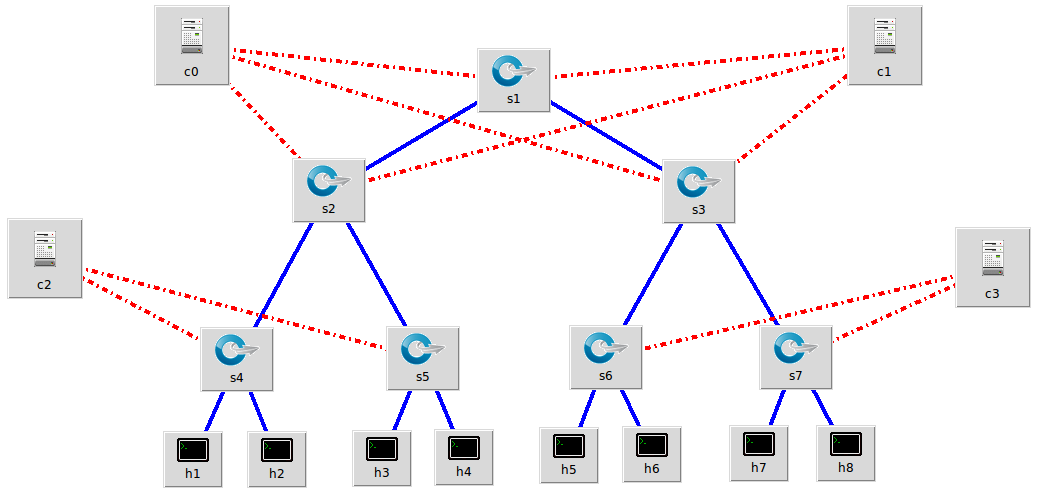
\includegraphics[width=1\linewidth]{img/challange-topology.png}
	\caption{the topology that you will have to implement in this activity, or rather
  a tree topology with multiple SDN controllers.
  The controllers \code{c2} and \code{c3} are local while \code{c0} and \code{c1}
  are remote controllers running on the same machine on which Mininet is running,
	listening respectively on TCP ports 6635 and 6636.}
	\label{fig:challenge-topology}
\end{figure}




\subsection*{Learning objectives}
After finishing this lab activity you will be able to apply what you have learnt
through the previous lab activities in order to implement on your own a given
topology which includes multiple controllers.





\subsection*{Scenario}
In this activity you will have to implement on your own the topology shown in
figure \ref{fig:challenge-topology} using the method you think is most appropriate
among those previously shown in this paper.

The activity is meant to let you test the knowledge you acquired through the
previous three activities proposed in this paper, therefore it assumes that you
have already completed them successfully.

The solution for this activity is available in the appendix A of this paper.



\subsection*{Task 1: implement the topology}
Implement the topology shown in figure \ref{fig:challenge-topology} using the method
you think is most appropriate.

\subsection*{Task 2: fix the network}
Assume that the controller \code{c3} failed and it's not working anymore: without
shutting down the whole network, fix the problem by connecting the switches served by \code{c3}
to the other available remote controller.
